\chapter{A new chapter} \label{chapter2}
Your second chapter probably has novel material in it. Hopefully. Here's a math object written using a shortcut that I defined in a separate file: $\Pzero$.

% Add additional \chapter{}s as necessary.

% use \cite{} to cite a reference in your bibliography file.
% use \ref{} to reference a \label{} from an equation, figure, or table.

% for sets of equations use align or gather:
%\begin{align}
%\end{align}

% for long equations, use multline.

% for figures:
\begin{figure}[ht]
\centering
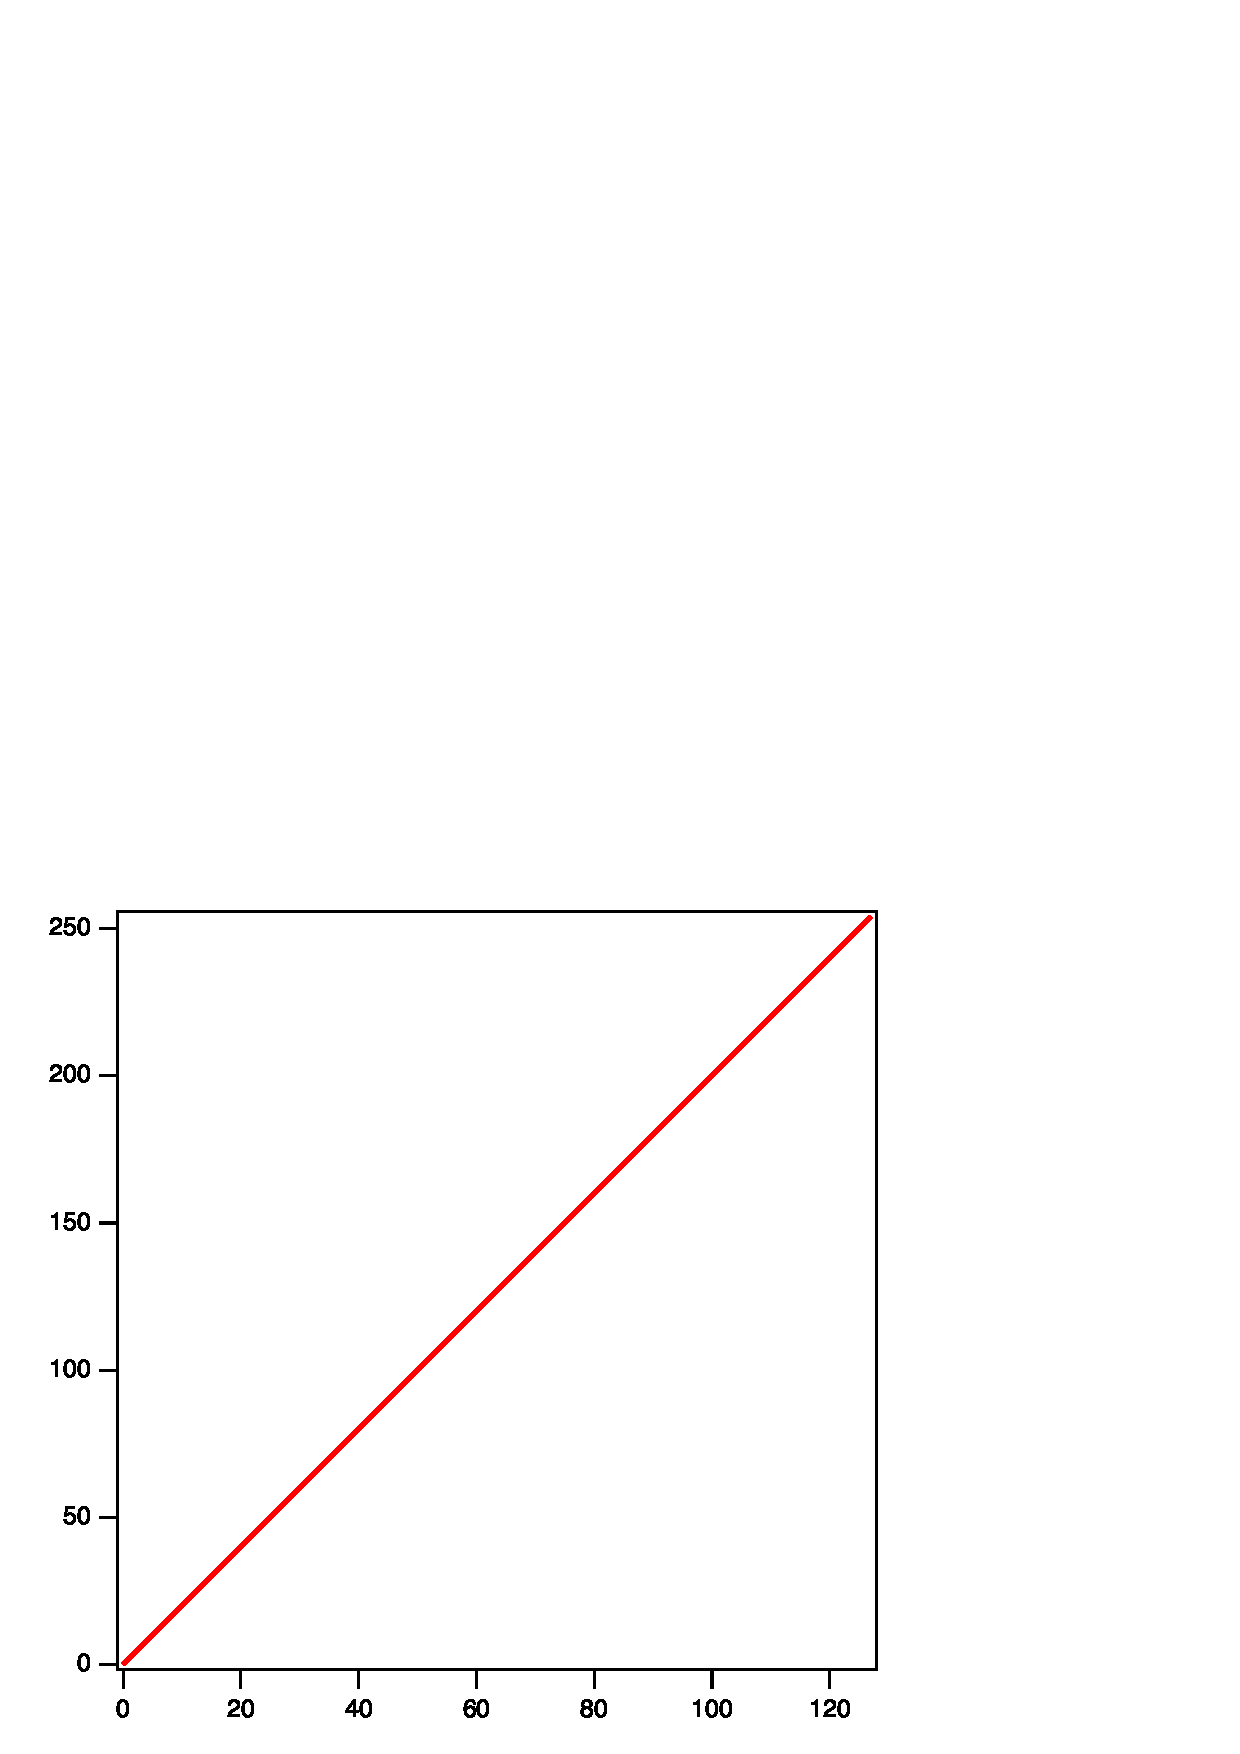
\includegraphics[width=.45\textwidth]{name_of_figure.pdf}
\caption[Short caption for the list of figures]{A figure caption!}
\label{a_figure}
\end{figure}

More material. Very exciting! Take a look at this reference to Figure~\ref{a_figure}.
Alternatively, you might want to use the \texttt{cleveref} package, which would give you this: \cref{a_figure}.
Or, you could use \texttt{hyperref}'s \texttt{autoref} command: \autoref{a_figure}.
I think that \texttt{cleveref} is the best of these options, because it lets you do multiple references gracefully and consistently: \cref{a_figure,a_table}.
\Cref{a_figure} can also be cited at the start of a sentence using \texttt{Cref} instead of \texttt{cref}; note the different result.

% for tables:
\begin{table}
\centering
\begin{tabular}{c|c|c}
 1 & 2 & 3 \\
 4 & 5 & 6 \\
 7 & 8 & 9 \\
\hline
\end{tabular}
\caption[Short caption for the list of tables]{Another caption! This one is for a table, not a figure.}
\label{a_table}
\end{table}
